\section{Patter Class Reference}
\label{classPatter}\index{Patter@{Patter}}
{\tt \#include $<$patter.h$>$}

Collaboration diagram for Patter:\begin{figure}[H]
\begin{center}
\leavevmode
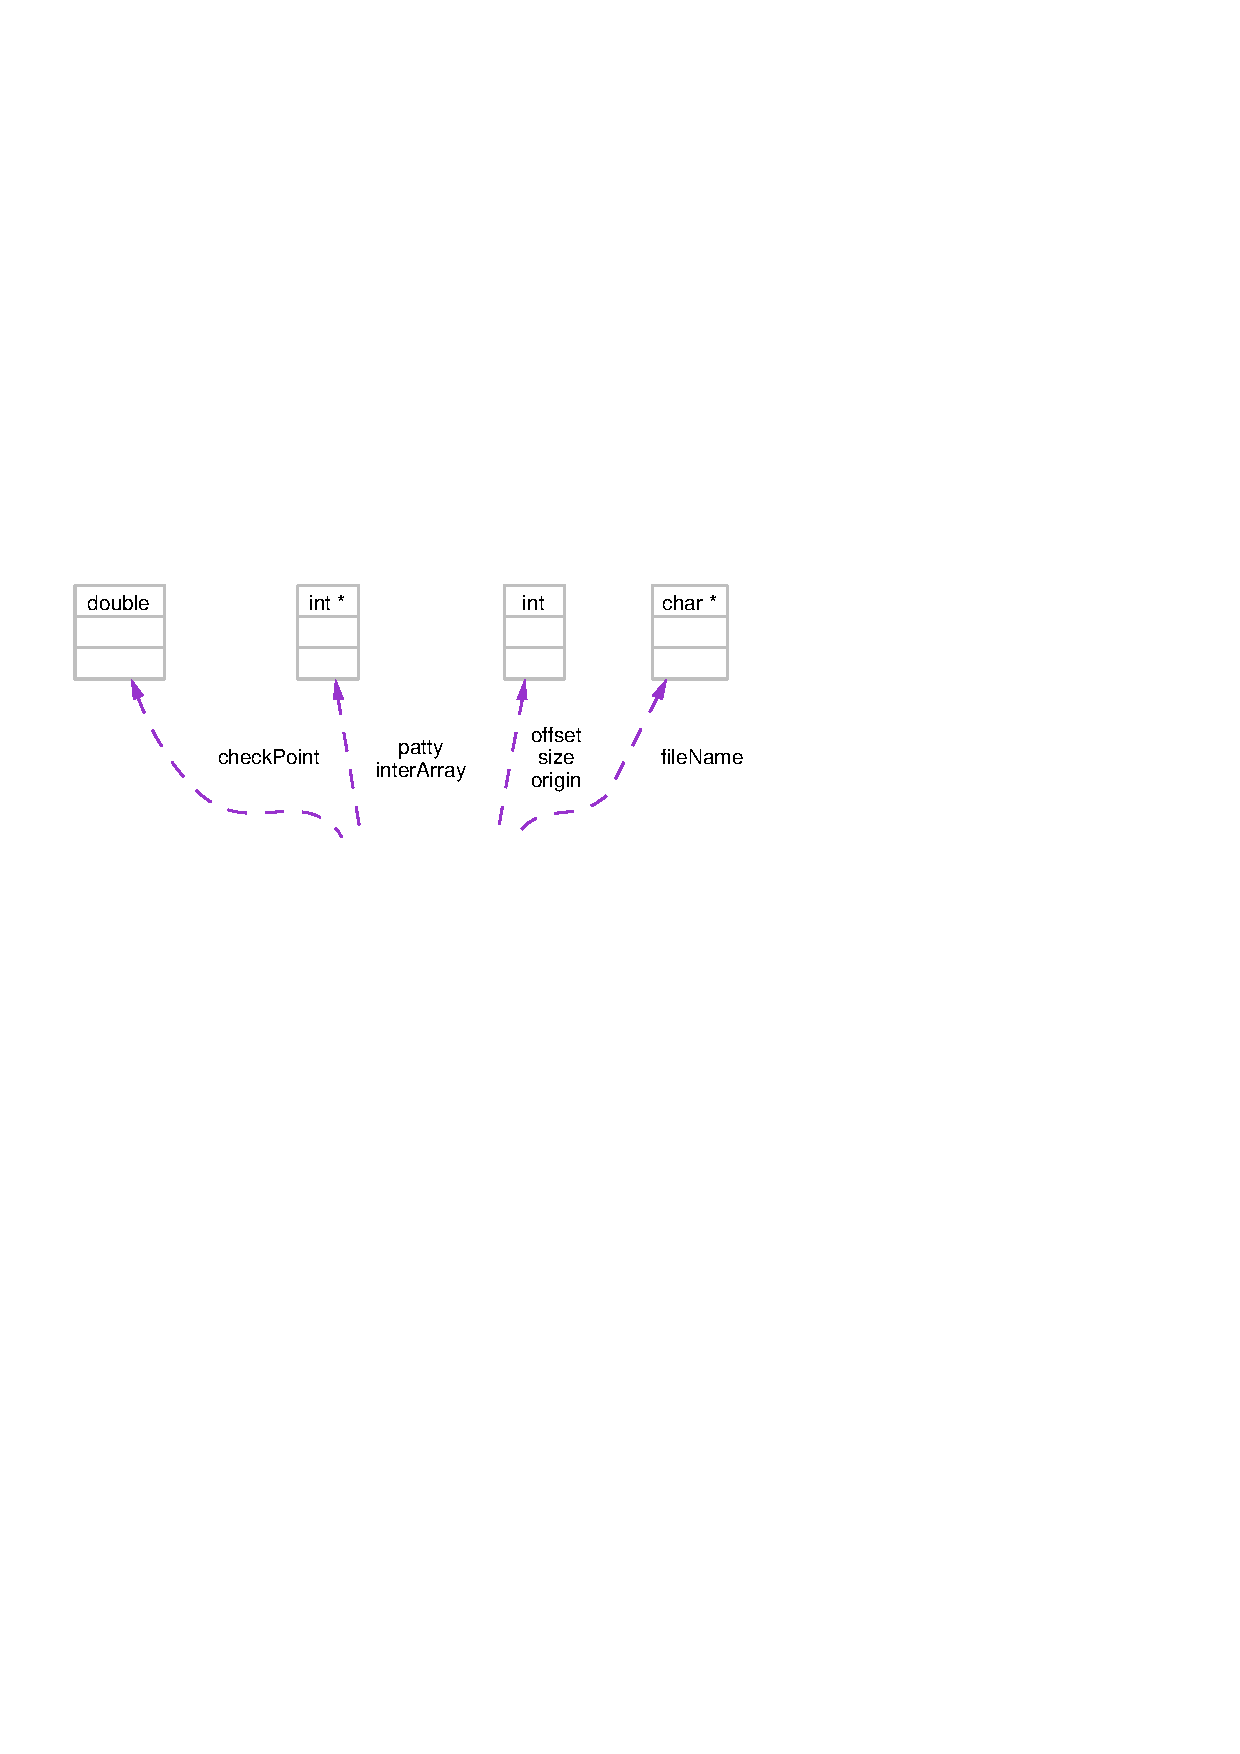
\includegraphics[width=194pt]{classPatter__coll__graph}
\end{center}
\end{figure}
\subsection*{Public Member Functions}
\begin{CompactItemize}
\item 
{\bf Patter} (char $\ast$a\-File)
\item 
{\bf Patter} (double a\-Check\-Point, int an\-Offset, char $\ast$a\-File)
\item 
{\bf Patter} (void)
\item 
{\bf $\sim$Patter} ()
\item 
void {\bf clear} ()
\item 
void {\bf Nursery} (int an\-Origin)
\item 
void {\bf Nursery} (std::list$<$ {\bf File\-Value} $>$ args)
\item 
int {\bf Delivery} (double {\bf check\-Point}, int {\bf offset})
\item 
void {\bf Get\-Patty} ()
\item 
std::list$<$ int $>$ {\bf get\-Pattern} (void)
\end{CompactItemize}
\subsection*{Private Member Functions}
\begin{CompactItemize}
\item 
void {\bf Init\-Pat} ()
\item 
void {\bf Init\-Pat} (int {\bf size}, int $\ast$data)
\item 
void {\bf Simple\-Pat} ()
\item 
void {\bf Init\-Prob} ()
\item 
void {\bf Expand} ()
\item 
void {\bf Expand} (std::list$<$ {\bf File\-Value} $>$ args)
\item 
void {\bf Equivalence} ()
\item 
void {\bf Equivalence} (int modulo, int low, int high)
\item 
void {\bf Symmetries} ()
\item 
void {\bf Symmetries} (int modulo, int low, int high)
\item 
void {\bf Distort} ()
\item 
void {\bf Distort} (int modulo, int low, int high)
\item 
void {\bf Adjust} ()
\item 
void {\bf Adjust} (int modulo, int low, int high)
\item 
bool {\bf Check\-Range} (int low, int high, int element)
\item 
int {\bf Chooser} (double {\bf check\-Point}, int {\bf offset})
\item 
void {\bf Recorder} (int file\-Length)
\end{CompactItemize}
\subsection*{Private Attributes}
\begin{CompactItemize}
\item 
int $\ast$ {\bf inter\-Array}
\item 
int $\ast$ {\bf patty}
\item 
int {\bf size}
\item 
int {\bf offset}
\item 
int {\bf origin}
\item 
double {\bf check\-Point}
\item 
char $\ast$ {\bf file\-Name}
\end{CompactItemize}


\subsection{Detailed Description}
This class generates a pattern of values using a user defined origin and a sequence of intervals and it delivers one value at a time. Same input may be used to generate various related paterns produced through mod m equivalences, symmetrical set forms (R, I, RI), and distortions. It uses input from user defined files describing the type of object and its parameters (box, sound, etc.) as well as the pattern itself (PAT file). \begin{Desc}
\item[Author:]Sever Tipei July 14, 2005 \end{Desc}




Definition at line 46 of file patter.h.

\subsection{Constructor \& Destructor Documentation}
\index{Patter@{Patter}!Patter@{Patter}}
\index{Patter@{Patter}!Patter@{Patter}}
\subsubsection{\setlength{\rightskip}{0pt plus 5cm}Patter::Patter (char $\ast$ {\em a\-File})}\label{classPatter_a0}


Constructor for (almost) empty object. File name PAT/... is necessary. 

Definition at line 49 of file patter.cpp.

References file\-Name, inter\-Array, patty, and size.\index{Patter@{Patter}!Patter@{Patter}}
\index{Patter@{Patter}!Patter@{Patter}}
\subsubsection{\setlength{\rightskip}{0pt plus 5cm}Patter::Patter (double {\em a\-Check\-Point}, int {\em an\-Offset}, char $\ast$ {\em a\-File})}\label{classPatter_a1}


Advanced constructor. 

Definition at line 60 of file patter.cpp.

References check\-Point, file\-Name, inter\-Array, offset, patty, and size.\index{Patter@{Patter}!Patter@{Patter}}
\index{Patter@{Patter}!Patter@{Patter}}
\subsubsection{\setlength{\rightskip}{0pt plus 5cm}Patter::Patter (void)}\label{classPatter_a2}


Constructor for empty object. This will be used by eventfactory system for evaluating patter objects. 

Definition at line 72 of file patter.cpp.

References inter\-Array, offset, origin, patty, and size.\index{Patter@{Patter}!~Patter@{$\sim$Patter}}
\index{~Patter@{$\sim$Patter}!Patter@{Patter}}
\subsubsection{\setlength{\rightskip}{0pt plus 5cm}Patter::$\sim${\bf Patter} ()}\label{classPatter_a3}


Destructor 

Definition at line 85 of file patter.cpp.

References clear().

Here is the call graph for this function:\begin{figure}[H]
\begin{center}
\leavevmode
\includegraphics[width=116pt]{classPatter_a3_cgraph}
\end{center}
\end{figure}


\subsection{Member Function Documentation}
\index{Patter@{Patter}!Adjust@{Adjust}}
\index{Adjust@{Adjust}!Patter@{Patter}}
\subsubsection{\setlength{\rightskip}{0pt plus 5cm}void Patter::Adjust (int {\em modulo}, int {\em low}, int {\em high})\hspace{0.3cm}{\tt  [private]}}\label{classPatter_d13}




Definition at line 499 of file patter.cpp.

References sever.\index{Patter@{Patter}!Adjust@{Adjust}}
\index{Adjust@{Adjust}!Patter@{Patter}}
\subsubsection{\setlength{\rightskip}{0pt plus 5cm}void Patter::Adjust ()\hspace{0.3cm}{\tt  [private]}}\label{classPatter_d12}




Definition at line 491 of file patter.cpp.

References sever.

Referenced by Delivery(), and Nursery().\index{Patter@{Patter}!CheckRange@{CheckRange}}
\index{CheckRange@{CheckRange}!Patter@{Patter}}
\subsubsection{\setlength{\rightskip}{0pt plus 5cm}bool Patter::Check\-Range (int {\em low}, int {\em high}, int {\em element})\hspace{0.3cm}{\tt  [private]}}\label{classPatter_d14}


Checks if the new element is within the defined range. 

Definition at line 508 of file patter.cpp.

Referenced by Equivalence().\index{Patter@{Patter}!Chooser@{Chooser}}
\index{Chooser@{Chooser}!Patter@{Patter}}
\subsubsection{\setlength{\rightskip}{0pt plus 5cm}int Patter::Chooser (double {\em check\-Point}, int {\em offset})\hspace{0.3cm}{\tt  [private]}}\label{classPatter_d15}


Coordinates various ways of choosing a member of the \_\-value\_\- array patty. 

Definition at line 516 of file patter.cpp.

References Data\-In::name\-Of, patty, Data\-In::Read\-Chars(), Read\-Compute\-Float(), and sever.

Referenced by Delivery().

Here is the call graph for this function:\begin{figure}[H]
\begin{center}
\leavevmode
\includegraphics[width=138pt]{classPatter_d15_cgraph}
\end{center}
\end{figure}
\index{Patter@{Patter}!clear@{clear}}
\index{clear@{clear}!Patter@{Patter}}
\subsubsection{\setlength{\rightskip}{0pt plus 5cm}void Patter::clear ()}\label{classPatter_a4}


Deletes pointer arrays. 

Definition at line 92 of file patter.cpp.

References inter\-Array, patty, and size.

Referenced by $\sim$Patter().\index{Patter@{Patter}!Delivery@{Delivery}}
\index{Delivery@{Delivery}!Patter@{Patter}}
\subsubsection{\setlength{\rightskip}{0pt plus 5cm}int Patter::Delivery (double {\em check\-Point}, int {\em offset})}\label{classPatter_a7}


Delivers the pattern array patty by calling various methods. Reads from the parent file. 

Definition at line 554 of file patter.cpp.

References Adjust(), Chooser(), Get\-Patty(), Data\-In::name\-Of, Data\-In::Read\-Chars(), Data\-In::Read\-Dummies(), and sever.

Here is the call graph for this function:\begin{figure}[H]
\begin{center}
\leavevmode
\includegraphics[width=207pt]{classPatter_a7_cgraph}
\end{center}
\end{figure}
\index{Patter@{Patter}!Distort@{Distort}}
\index{Distort@{Distort}!Patter@{Patter}}
\subsubsection{\setlength{\rightskip}{0pt plus 5cm}void Patter::Distort (int {\em modulo}, int {\em low}, int {\em high})\hspace{0.3cm}{\tt  [private]}}\label{classPatter_d11}




Definition at line 480 of file patter.cpp.

References sever.\index{Patter@{Patter}!Distort@{Distort}}
\index{Distort@{Distort}!Patter@{Patter}}
\subsubsection{\setlength{\rightskip}{0pt plus 5cm}void Patter::Distort ()\hspace{0.3cm}{\tt  [private]}}\label{classPatter_d10}




Definition at line 471 of file patter.cpp.

References sever.

Referenced by Expand().\index{Patter@{Patter}!Equivalence@{Equivalence}}
\index{Equivalence@{Equivalence}!Patter@{Patter}}
\subsubsection{\setlength{\rightskip}{0pt plus 5cm}void Patter::Equivalence (int {\em modulo}, int {\em low}, int {\em high})\hspace{0.3cm}{\tt  [private]}}\label{classPatter_d7}




Definition at line 396 of file patter.cpp.

References Check\-Range(), Random::Choose\-From\-Prob(), Cumul\-Array(), inter\-Array, origin, patty, and size.

Here is the call graph for this function:\begin{figure}[H]
\begin{center}
\leavevmode
\includegraphics[width=260pt]{classPatter_d7_cgraph}
\end{center}
\end{figure}
\index{Patter@{Patter}!Equivalence@{Equivalence}}
\index{Equivalence@{Equivalence}!Patter@{Patter}}
\subsubsection{\setlength{\rightskip}{0pt plus 5cm}void Patter::Equivalence ()\hspace{0.3cm}{\tt  [private]}}\label{classPatter_d6}


Finds all intervals allowed by a given range which are equivalent mod m with the initial list. The \char`\"{}num\-Terms\char`\"{} equivalence should not be reduced since the terms are integers.

do devise other ways of assigning probabilities to equivalence clases. 

Definition at line 333 of file patter.cpp.

References Check\-Range(), Random::Choose\-From\-Prob(), Cumul\-Array(), inter\-Array, Data\-In::int\-Vect, origin, patty, Data\-In::Read\-Ints(), and size.

Referenced by Expand().

Here is the call graph for this function:\begin{figure}[H]
\begin{center}
\leavevmode
\includegraphics[width=260pt]{classPatter_d6_cgraph}
\end{center}
\end{figure}
\index{Patter@{Patter}!Expand@{Expand}}
\index{Expand@{Expand}!Patter@{Patter}}
\subsubsection{\setlength{\rightskip}{0pt plus 5cm}void Patter::Expand (std::list$<$ {\bf File\-Value} $>$ {\em args})\hspace{0.3cm}{\tt  [private]}}\label{classPatter_d5}




Definition at line 296 of file patter.cpp.

References Distort(), Equivalence(), sever, and Symmetries().

Here is the call graph for this function:\begin{figure}[H]
\begin{center}
\leavevmode
\includegraphics[width=318pt]{classPatter_d5_cgraph}
\end{center}
\end{figure}
\index{Patter@{Patter}!Expand@{Expand}}
\index{Expand@{Expand}!Patter@{Patter}}
\subsubsection{\setlength{\rightskip}{0pt plus 5cm}void Patter::Expand ()\hspace{0.3cm}{\tt  [private]}}\label{classPatter_d4}


Coordinates various methos of expanding and/or modifying the pattern: equivalence classes, transpositions, symmetric forms (I, R, RI), distortions (augmentation, diminution, etc,), etc. 

Definition at line 266 of file patter.cpp.

References Distort(), Equivalence(), Data\-In::name\-Of, Data\-In::Read\-Chars(), sever, and Symmetries().

Referenced by Nursery().

Here is the call graph for this function:\begin{figure}[H]
\begin{center}
\leavevmode
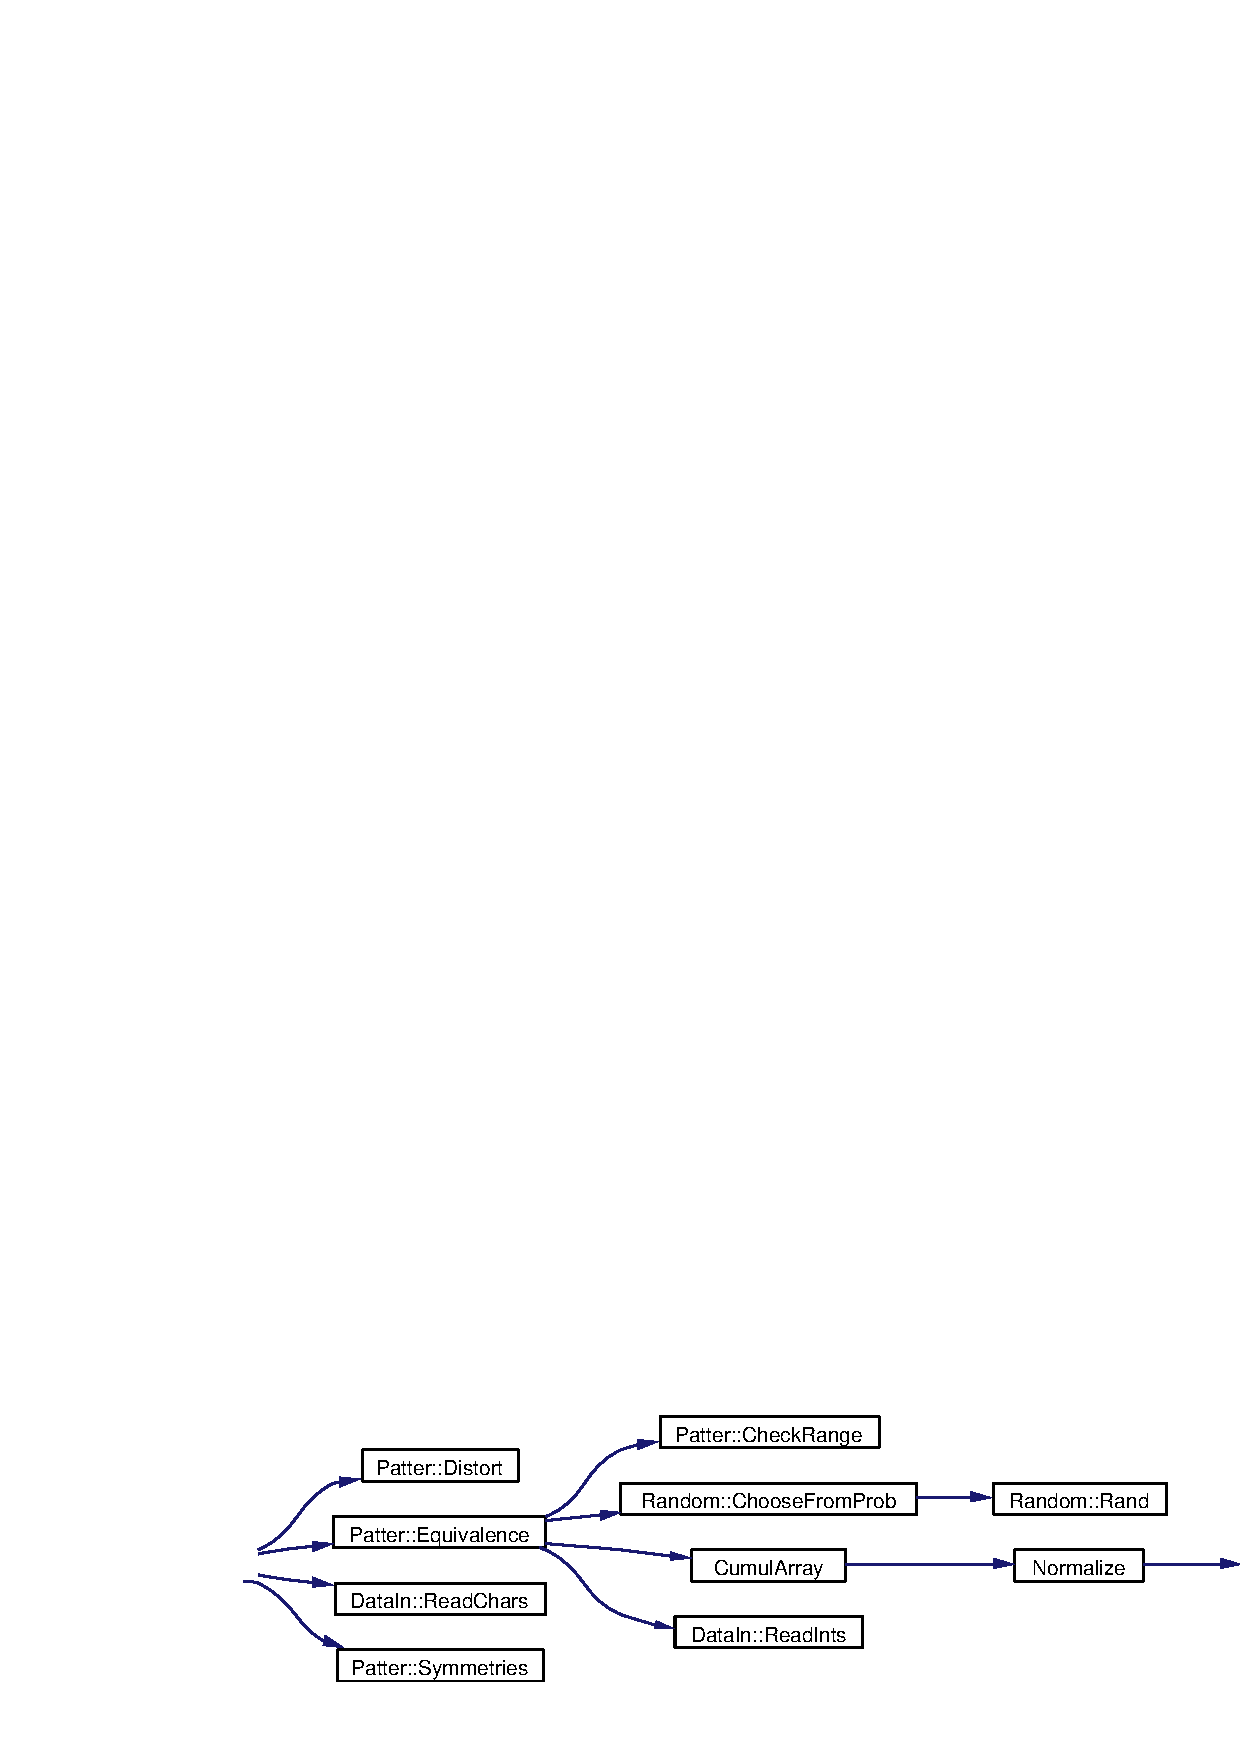
\includegraphics[width=318pt]{classPatter_d4_cgraph}
\end{center}
\end{figure}
\index{Patter@{Patter}!getPattern@{getPattern}}
\index{getPattern@{getPattern}!Patter@{Patter}}
\subsubsection{\setlength{\rightskip}{0pt plus 5cm}std::list$<$ int $>$ Patter::get\-Pattern (void)}\label{classPatter_a9}


Return a pattern object created by \char`\"{}Nursery\char`\"{} via the eventfactory interface. 

Definition at line 649 of file patter.cpp.

References patty, and size.

Referenced by File\-Value::Evaluate().\index{Patter@{Patter}!GetPatty@{GetPatty}}
\index{GetPatty@{GetPatty}!Patter@{Patter}}
\subsubsection{\setlength{\rightskip}{0pt plus 5cm}void Patter::Get\-Patty ()}\label{classPatter_a8}


Reads an existing pattern from a PAT file (at the end of the file) created by a previous Patter object and stores it in an array (patty) to be used by the current Patter object. It is called only for objects (eg. sounds) whose numbers are $>$ 0, not by the first object in a series. 

Definition at line 587 of file patter.cpp.

References Data\-In::Gen\-Ints(), Data\-In::g\-Int\-Vect, Data\-In::int\-Vect, patty, Data\-In::Read\-Dummies(), Data\-In::Read\-Ints(), size, and Data\-In::Skip().

Referenced by Delivery().

Here is the call graph for this function:\begin{figure}[H]
\begin{center}
\leavevmode
\includegraphics[width=147pt]{classPatter_a8_cgraph}
\end{center}
\end{figure}
\index{Patter@{Patter}!InitPat@{InitPat}}
\index{InitPat@{InitPat}!Patter@{Patter}}
\subsubsection{\setlength{\rightskip}{0pt plus 5cm}void Patter::Init\-Pat (int {\em size}, int $\ast$ {\em data})\hspace{0.3cm}{\tt  [private]}}\label{classPatter_d1}




Definition at line 212 of file patter.cpp.

References inter\-Array, patty, and size.\index{Patter@{Patter}!InitPat@{InitPat}}
\index{InitPat@{InitPat}!Patter@{Patter}}
\subsubsection{\setlength{\rightskip}{0pt plus 5cm}void Patter::Init\-Pat ()\hspace{0.3cm}{\tt  [private]}}\label{classPatter_d0}


Creates an empty array patty. Reads in an \_\-interval\_\- pattern from a PAT file and copies it into an array of intervals which can be manipulated further. 

Definition at line 191 of file patter.cpp.

References Data\-In::Gen\-Ints(), Data\-In::g\-Int\-Vect, inter\-Array, Data\-In::int\-Vect, patty, Data\-In::Read\-Ints(), and size.

Referenced by Nursery().

Here is the call graph for this function:\begin{figure}[H]
\begin{center}
\leavevmode
\includegraphics[width=126pt]{classPatter_d0_cgraph}
\end{center}
\end{figure}
\index{Patter@{Patter}!InitProb@{InitProb}}
\index{InitProb@{InitProb}!Patter@{Patter}}
\subsubsection{\setlength{\rightskip}{0pt plus 5cm}void Patter::Init\-Prob ()\hspace{0.3cm}{\tt  [private]}}\label{classPatter_d3}




Definition at line 246 of file patter.cpp.

Referenced by Nursery().\index{Patter@{Patter}!Nursery@{Nursery}}
\index{Nursery@{Nursery}!Patter@{Patter}}
\subsubsection{\setlength{\rightskip}{0pt plus 5cm}void Patter::Nursery (std::list$<$ {\bf File\-Value} $>$ {\em args})}\label{classPatter_a6}




Definition at line 143 of file patter.cpp.

References Adjust(), Expand(), Init\-Pat(), Init\-Prob(), sever, Simple\-Pat(), and size.

Here is the call graph for this function:\begin{figure}[H]
\begin{center}
\leavevmode
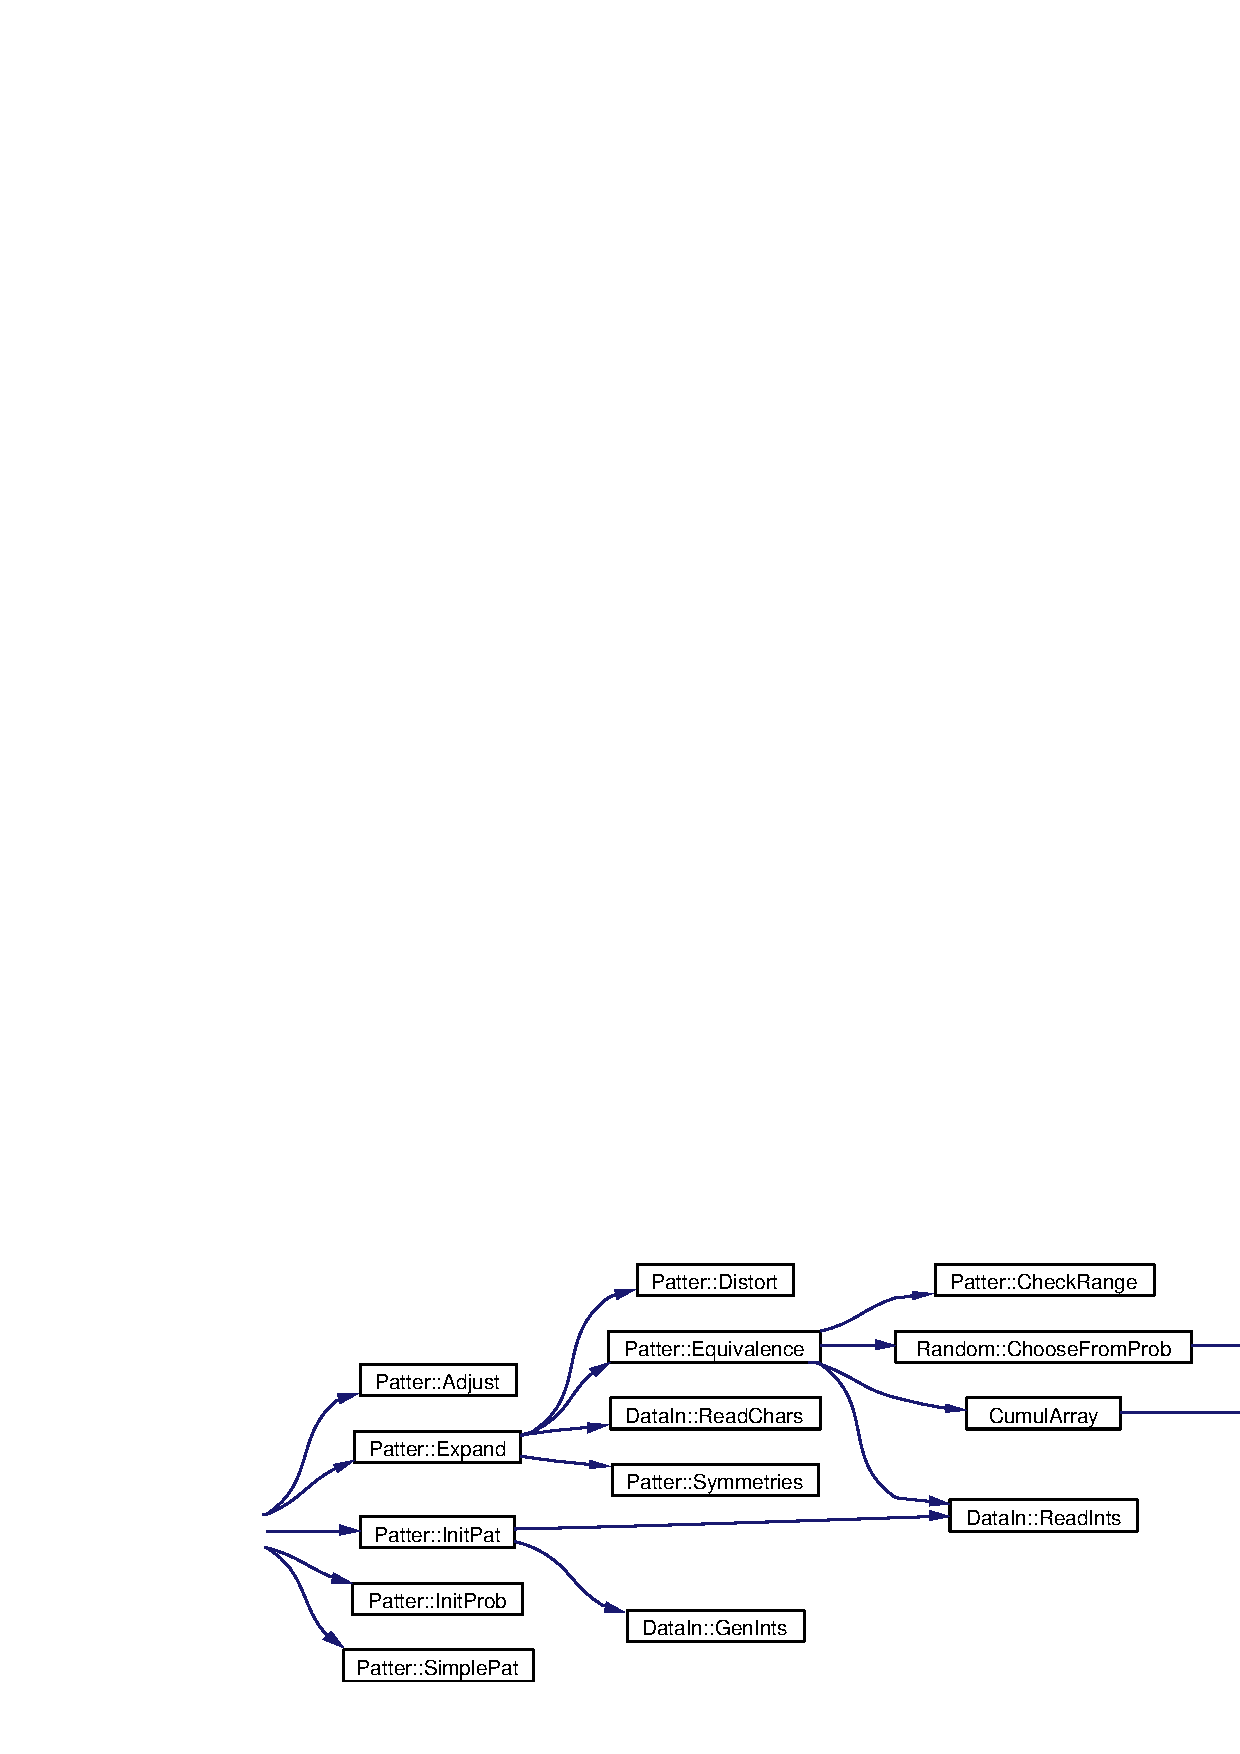
\includegraphics[width=384pt]{classPatter_a6_cgraph}
\end{center}
\end{figure}
\index{Patter@{Patter}!Nursery@{Nursery}}
\index{Nursery@{Nursery}!Patter@{Patter}}
\subsubsection{\setlength{\rightskip}{0pt plus 5cm}void Patter::Nursery (int {\em an\-Origin})}\label{classPatter_a5}


Coordinates the creation of a new pattern from data in a PAT file by calling various methods. Records the new pattern at the end of the PAT file. It is called only for the first object in a series of similar objects. 

Definition at line 101 of file patter.cpp.

References Adjust(), Expand(), Init\-Pat(), Init\-Prob(), Data\-In::int\-Vect, Data\-In::name\-Of, origin, Data\-In::Read\-Chars(), Data\-In::Read\-Dummies(), Data\-In::Read\-Ints(), Recorder(), sever, and Simple\-Pat().

Referenced by File\-Value::Evaluate().

Here is the call graph for this function:\begin{figure}[H]
\begin{center}
\leavevmode
\includegraphics[width=401pt]{classPatter_a5_cgraph}
\end{center}
\end{figure}
\index{Patter@{Patter}!Recorder@{Recorder}}
\index{Recorder@{Recorder}!Patter@{Patter}}
\subsubsection{\setlength{\rightskip}{0pt plus 5cm}void Patter::Recorder (int {\em file\-Length})\hspace{0.3cm}{\tt  [private]}}\label{classPatter_d16}


Records a pattern created by \char`\"{}Nursery\char`\"{} at the end of a PAT file. It copies the content of the PAT file up to the pattern into a buffer array, opens an output file with the same name as the original (input) file and writes first the content of the original file and then the pattern array patty. This way, if the same pattern file is used multiple times to generate similar patterns, only the record of the current patty array is kept. 

Definition at line 610 of file patter.cpp.

References Data\-In::buffer, file\-Name, patty, Data\-In::Read\-Buffer(), Data\-In::rewind\-File(), and size.

Referenced by Nursery().

Here is the call graph for this function:\begin{figure}[H]
\begin{center}
\leavevmode
\includegraphics[width=141pt]{classPatter_d16_cgraph}
\end{center}
\end{figure}
\index{Patter@{Patter}!SimplePat@{SimplePat}}
\index{SimplePat@{SimplePat}!Patter@{Patter}}
\subsubsection{\setlength{\rightskip}{0pt plus 5cm}void Patter::Simple\-Pat ()\hspace{0.3cm}{\tt  [private]}}\label{classPatter_d2}


Creates a patty array by starting with the origin and adding to each location the next member of the interval array inter\-Array 

Definition at line 229 of file patter.cpp.

References inter\-Array, origin, patty, and size.

Referenced by Nursery().\index{Patter@{Patter}!Symmetries@{Symmetries}}
\index{Symmetries@{Symmetries}!Patter@{Patter}}
\subsubsection{\setlength{\rightskip}{0pt plus 5cm}void Patter::Symmetries (int {\em modulo}, int {\em low}, int {\em high})\hspace{0.3cm}{\tt  [private]}}\label{classPatter_d9}




Definition at line 462 of file patter.cpp.

References sever.\index{Patter@{Patter}!Symmetries@{Symmetries}}
\index{Symmetries@{Symmetries}!Patter@{Patter}}
\subsubsection{\setlength{\rightskip}{0pt plus 5cm}void Patter::Symmetries ()\hspace{0.3cm}{\tt  [private]}}\label{classPatter_d8}




Definition at line 454 of file patter.cpp.

References sever.

Referenced by Expand().

\subsection{Member Data Documentation}
\index{Patter@{Patter}!checkPoint@{checkPoint}}
\index{checkPoint@{checkPoint}!Patter@{Patter}}
\subsubsection{\setlength{\rightskip}{0pt plus 5cm}double {\bf Patter::check\-Point}\hspace{0.3cm}{\tt  [private]}}\label{classPatter_r5}




Definition at line 200 of file patter.h.

Referenced by Patter().\index{Patter@{Patter}!fileName@{fileName}}
\index{fileName@{fileName}!Patter@{Patter}}
\subsubsection{\setlength{\rightskip}{0pt plus 5cm}char$\ast$ {\bf Patter::file\-Name}\hspace{0.3cm}{\tt  [private]}}\label{classPatter_r6}




Definition at line 202 of file patter.h.

Referenced by Patter(), and Recorder().\index{Patter@{Patter}!interArray@{interArray}}
\index{interArray@{interArray}!Patter@{Patter}}
\subsubsection{\setlength{\rightskip}{0pt plus 5cm}int$\ast$ {\bf Patter::inter\-Array}\hspace{0.3cm}{\tt  [private]}}\label{classPatter_r0}




Definition at line 194 of file patter.h.

Referenced by clear(), Equivalence(), Init\-Pat(), Patter(), and Simple\-Pat().\index{Patter@{Patter}!offset@{offset}}
\index{offset@{offset}!Patter@{Patter}}
\subsubsection{\setlength{\rightskip}{0pt plus 5cm}int {\bf Patter::offset}\hspace{0.3cm}{\tt  [private]}}\label{classPatter_r3}




Definition at line 198 of file patter.h.

Referenced by Patter().\index{Patter@{Patter}!origin@{origin}}
\index{origin@{origin}!Patter@{Patter}}
\subsubsection{\setlength{\rightskip}{0pt plus 5cm}int {\bf Patter::origin}\hspace{0.3cm}{\tt  [private]}}\label{classPatter_r4}




Definition at line 199 of file patter.h.

Referenced by Equivalence(), Nursery(), Patter(), and Simple\-Pat().\index{Patter@{Patter}!patty@{patty}}
\index{patty@{patty}!Patter@{Patter}}
\subsubsection{\setlength{\rightskip}{0pt plus 5cm}int$\ast$ {\bf Patter::patty}\hspace{0.3cm}{\tt  [private]}}\label{classPatter_r1}




Definition at line 195 of file patter.h.

Referenced by Chooser(), clear(), Equivalence(), get\-Pattern(), Get\-Patty(), Init\-Pat(), Patter(), Recorder(), and Simple\-Pat().\index{Patter@{Patter}!size@{size}}
\index{size@{size}!Patter@{Patter}}
\subsubsection{\setlength{\rightskip}{0pt plus 5cm}int {\bf Patter::size}\hspace{0.3cm}{\tt  [private]}}\label{classPatter_r2}




Definition at line 197 of file patter.h.

Referenced by clear(), Equivalence(), get\-Pattern(), Get\-Patty(), Init\-Pat(), Nursery(), Patter(), Recorder(), and Simple\-Pat().

The documentation for this class was generated from the following files:\begin{CompactItemize}
\item 
{\bf patter.h}\item 
{\bf patter.cpp}\end{CompactItemize}
